\documentclass{sigchi}

% Use this command to override the default ACM copyright statement (e.g. for preprints). 
% Consult the conference website for the camera-ready copyright statement.


%% EXAMPLE BEGIN -- HOW TO OVERRIDE THE DEFAULT COPYRIGHT STRIP -- (July 22, 2013 - Paul Baumann)
% \toappear{Permission to make digital or hard copies of all or part of this work for personal or classroom use is  granted without fee provided that copies are not made or distributed for profit or commercial advantage and that copies bear this notice and the full citation on the first page. Copyrights for components of this work owned by others than ACM must be honored. Abstracting with credit is permitted. To copy otherwise, or republish, to post on servers or to redistribute to lists, requires prior specific permission and/or a fee. Request permissions from permissions@acm.org. \\
% {\emph{CHI'14}}, April 26--May 1, 2014, Toronto, Canada. \\
% Copyright \copyright~2014 ACM ISBN/14/04...\$15.00. \\
% DOI string from ACM form confirmation}
%% EXAMPLE END -- HOW TO OVERRIDE THE DEFAULT COPYRIGHT STRIP -- (July 22, 2013 - Paul Baumann)


% Arabic page numbers for submission. 
% Remove this line to eliminate page numbers for the camera ready copy
\pagenumbering{arabic}


% Load basic packages
\usepackage{balance}  % to better equalize the last page
\usepackage{graphics} % for EPS, load graphicx instead
\usepackage{times}    % comment if you want LaTeX's default font
\usepackage{url}      % llt: nicely formatted URLs

% llt: Define a global style for URLs, rather that the default one
\makeatletter
\def\url@leostyle{%
  \@ifundefined{selectfont}{\def\UrlFont{\sf}}{\def\UrlFont{\small\bf\ttfamily}}}
\makeatother
\urlstyle{leo}


% To make various LaTeX processors do the right thing with page size.
\def\pprw{8.5in}
\def\pprh{11in}
\special{papersize=\pprw,\pprh}
\setlength{\paperwidth}{\pprw}
\setlength{\paperheight}{\pprh}
\setlength{\pdfpagewidth}{\pprw}
\setlength{\pdfpageheight}{\pprh}

% Make sure hyperref comes last of your loaded packages, 
% to give it a fighting chance of not being over-written, 
% since its job is to redefine many LaTeX commands.
\usepackage[pdftex]{hyperref}
\hypersetup{
pdftitle={SIGCHI Conference Proceedings Format},
pdfauthor={LaTeX},
pdfkeywords={SIGCHI, proceedings, archival format},
bookmarksnumbered,
pdfstartview={FitH},
colorlinks,
citecolor=black,
filecolor=black,
linkcolor=black,
urlcolor=black,
breaklinks=true,
}

% create a shortcut to typeset table headings
\newcommand\tabhead[1]{\small\textbf{#1}}


% End of preamble. Here it comes the document.
\begin{document}

\title{Hello! Foreigner: Using Body Language Communication in Cooperative Game Design}

\numberofauthors{6}
\author{
  \alignauthor 1st Author Name\\
    \affaddr{Affiliation}\\
    \affaddr{Address}\\
    \email{e-mail address}\\
    \affaddr{Optional phone number}
  \alignauthor 2nd Author Name\\
    \affaddr{Affiliation}\\
    \affaddr{Address}\\
    \email{e-mail address}\\
    \affaddr{Optional phone number}    
  \alignauthor 3rd Author Name\\
    \affaddr{Affiliation}\\
    \affaddr{Address}\\
    \email{e-mail address}\\
    \affaddr{Optional phone number}
  \alignauthor 4th Author Name\\
    \affaddr{Affiliation}\\
    \affaddr{Address}\\
    \email{e-mail address}\\
    \affaddr{Optional phone number}
  \alignauthor 5th Author Name\\
    \affaddr{Affiliation}\\
    \affaddr{Address}\\
    \email{e-mail address}\\
    \affaddr{Optional phone number}
  \alignauthor 6th Author Name\\
    \affaddr{Affiliation}\\
    \affaddr{Address}\\
    \email{e-mail address}\\
    \affaddr{Optional phone number}    
}

\maketitle

\begin{abstract}


In this work, we want to explore the game design for body language communication in cooperative game. With this purpose, we propose design goals we wish to achieve. Afterwards, by following our game design goal, we complete a game prototype, Mute Robot, which is used to evaluate and confirm our thoughts. According to our user study results, fun and enjoyment of the game are 4.5(on a scale of 1 to 5), and have quite great co-experience. Last but not least, we offer the design guidelines for body language communication in cooperative games.

% Second, follow our game goals, we make a game prototype, Mute Robot, to evaluate and confirm our thoughts. The results of the user study are excellent, and the game fun and enjoyment are 4.5(on a scale of 1 to 5), and have quite good co-experience. Finally, we propose the design guidelines for body language communication in cooperative game.

\end{abstract}

\keywords{
  game design; body language; cooperative game; interaction; video games; kinect
  % Guides; instructions; author's kit; conference publications;
  % keywords should be separated by a semi-colon.
  % \textcolor{red}{Mandatory section to be included in your final version.}
}

\category{H.5.m.}{Information Interfaces and Presentation (e.g. HCI)}{Miscellaneous}

% See: \url{http://www.acm.org/about/class/1998/}
% for more information and the full list of ACM classifiers
% and descriptors. 
% \textcolor{red}{Mandatory section to be included in your
% final version. On the submission page only the classifiers'
% letter-number combination will need to be entered.}

\section{Introduction}

In the last decades, cooperation has developed from an additional feature into a full-grown game component, motivating more and more players to join a game. As a result, there is more and more researchers study in cooperative game design. Based on previous works, we explore the possibility of using body language in cooperative game design. Because body language is a universal language that everyone use naturally, we believe it is suitable for cooperative game which needs intensive communication with partners.

We think out some design goals for body language communication, and develop a prototype game, Mute Robot, to evaluate player's game experience. We follow the goals to design our game prototype. Then we conduct user study by recruiting 24 groups within 48 users. Depending on our user study results, we can confirm that our game design for body language communication is quite successful. In final, in order to consider our observations and user feedback, we propose ten design guidelines and expect it is beneficial for people who want to study body language communication in game design in the future. 

% \begin{figure}[!h]
% \centering
% \includegraphics[width=0.9\columnwidth]{Figure11}
% \caption{With Caption Below, be sure to have a good resolution image
%   (see item D within the preparation instructions).}
% \label{fig:figure1}
% \end{figure}

\section{Related Work}
\subsection{Non-verbal communication game}

Cooperative games with nonverbal communication had hit the market in these years. Players in Journey, the best game of the year in GDC 2013 \cite{I0}, can only communicate with each other by giving off pleasant sounds; Another game, Ways, allows player to use the mouse and the keyboard to control their avatar's posture to communicate with each other. And the other game, Dark Souls, which is a famous game sold over 2.61 million copies, can only communicate through a set of predefined character animation.

Nonverbal communication systems had already existed and had been studied earlier. 
Galentucci \cite{I1} has designed a setting, which needs two players, located in different places, to play video games with communication requirement.
% Galentucci [7] has looked at a setting where pairs located in different places were playing video games that required communication. 
They could communicate through graphical signals without using letters, and sign languages will be developed during the game; 
Innocent and Haines \cite{I2} has been developed and evaluated a system called ``symbolchat'', which is used in online multiplayer game worlds. In some research, a large set of symbols has been developed to be used for communication so that the symbol set becomes to resemble a language \cite{I3,I4}. Beyond pictographic chat systems, Åkerman et al. \cite{I5} also presented a gameboard for players to communicate through picture drawing. In our work, we explore and evaluate the possibility to use body language as a communication manner in cooperative game design, which becomes a new nonverbal communication manner for gaming.

\subsection{Cooperative Game Design}

Some researchers had already developed cooperative game design patterns. For example, Zagal et al. explored cooperative patterns within board games \cite{CG1}. Bjork and Holopainen presented a large quantity of game design patterns \cite{CG3}. Rocha et al. \cite{CG4} proposed a framework of several cooperative game design patterns. El-Nasr et al. \cite{CPMs} extended the cooperative game design proposed from Rocha, and presented a Cooperative Performance Metrics(CPM) used for analysis of cooperative games. We refered works mentioned above, and proposed new design patterns for body language communication in cooperative game.

\section{Design Goal}
In order to make significant design and contribution, we defined following goals for us to approach and achieve before game design.

\begin{enumerate}
\item Focus on Communication: a body language communication game without body language communication just makes no sense. So we think communication should be required in each level. For communication game, the most important thing is communication rather than manipulation.

\item Test the limitation: we want to test the limitation and find out all possibility of using body language in cooperative games.
For this reason, the concept of each game level is distinct and progressive.
% 因此每個遊戲階段需要表達的概念應該是不一樣的,並且是漸進式的,慢慢加深,挖掘body language的所有可能性。
% we desire to explore the limitation of using body language as communication manner in the cooperative game. 
Therefore, in our game prototype, there are three stages with three different types of informations needed to be passed in the game. 
% The difficulty increases 

\item Cooperative Fun: 
we anticipate players can interact with each other by their body and limbs and strengthen players' collaborative experience. While playing the game, players can build up an effective connection and both of them can have deeper recognition with each other.
% 我們期望借由肢體上的互動,可以加強玩家間的合作體驗,並在遊玩的過程中建立情感的聯結,遊玩結束後能對一起玩的夥伴有更深的認識。
% With virtual physical interaction between two players, they can build up the connection of emotion and have more knowledge about their partners after the game ends. 

\item Avoid Frustration: 
we think using body language can resolve the communication obstacle if there is language barrier between players. Body language also can decrease frustration by the matter of communication and produce better gameplay experience.
% 期望透過肢體語言可以解決語言不通的玩家在遊玩時的溝通障礙,降低因為溝通的問題所產生的挫折感,使遊戲體驗不會受到影響。
% Without common language between players causes the frustration when players communicate with each other. However, 

\item University: we want to make a better environment. If one day, all people around the world can play a cooperative game through body language, it means that we succeed in decreasing the limitation of language barrier significantly.
% 所有人都可以透過body language進行遊戲,儘量降低語言上的限制。
\end{enumerate}

\section{Implementation}

Follow the design goals we proposed, we design a game prototype Mute Robot.

\subsection{Game Prototype - Mute Robot}

The main idea we want to explore is the game design of using body language in a cooperative game. In order to find out the answer, we had designed Mute Robot, a game in which two players must cooperate to solve a series of puzzle challenges by communicating through body language only.

Mute Robot is a cooperative puzzle platformer game built using Unity3D \cite{unity} engine. The game involves two players at two distinct locations connected over the Internet. The players cannot talk to each other directly and the only way to communicate is using their body language. We use Kinect (v1) to capture player’s body language and apply to their avatar(see Figure \ref{fig:GD_F1}). In order to avoid arm fatigue of mid-air interactions with Kinect, each player uses a Wii controller to completely trivial manipulation (e.g. move left, move right, confirm, cancel).  

\begin{figure}[!h]
\centering
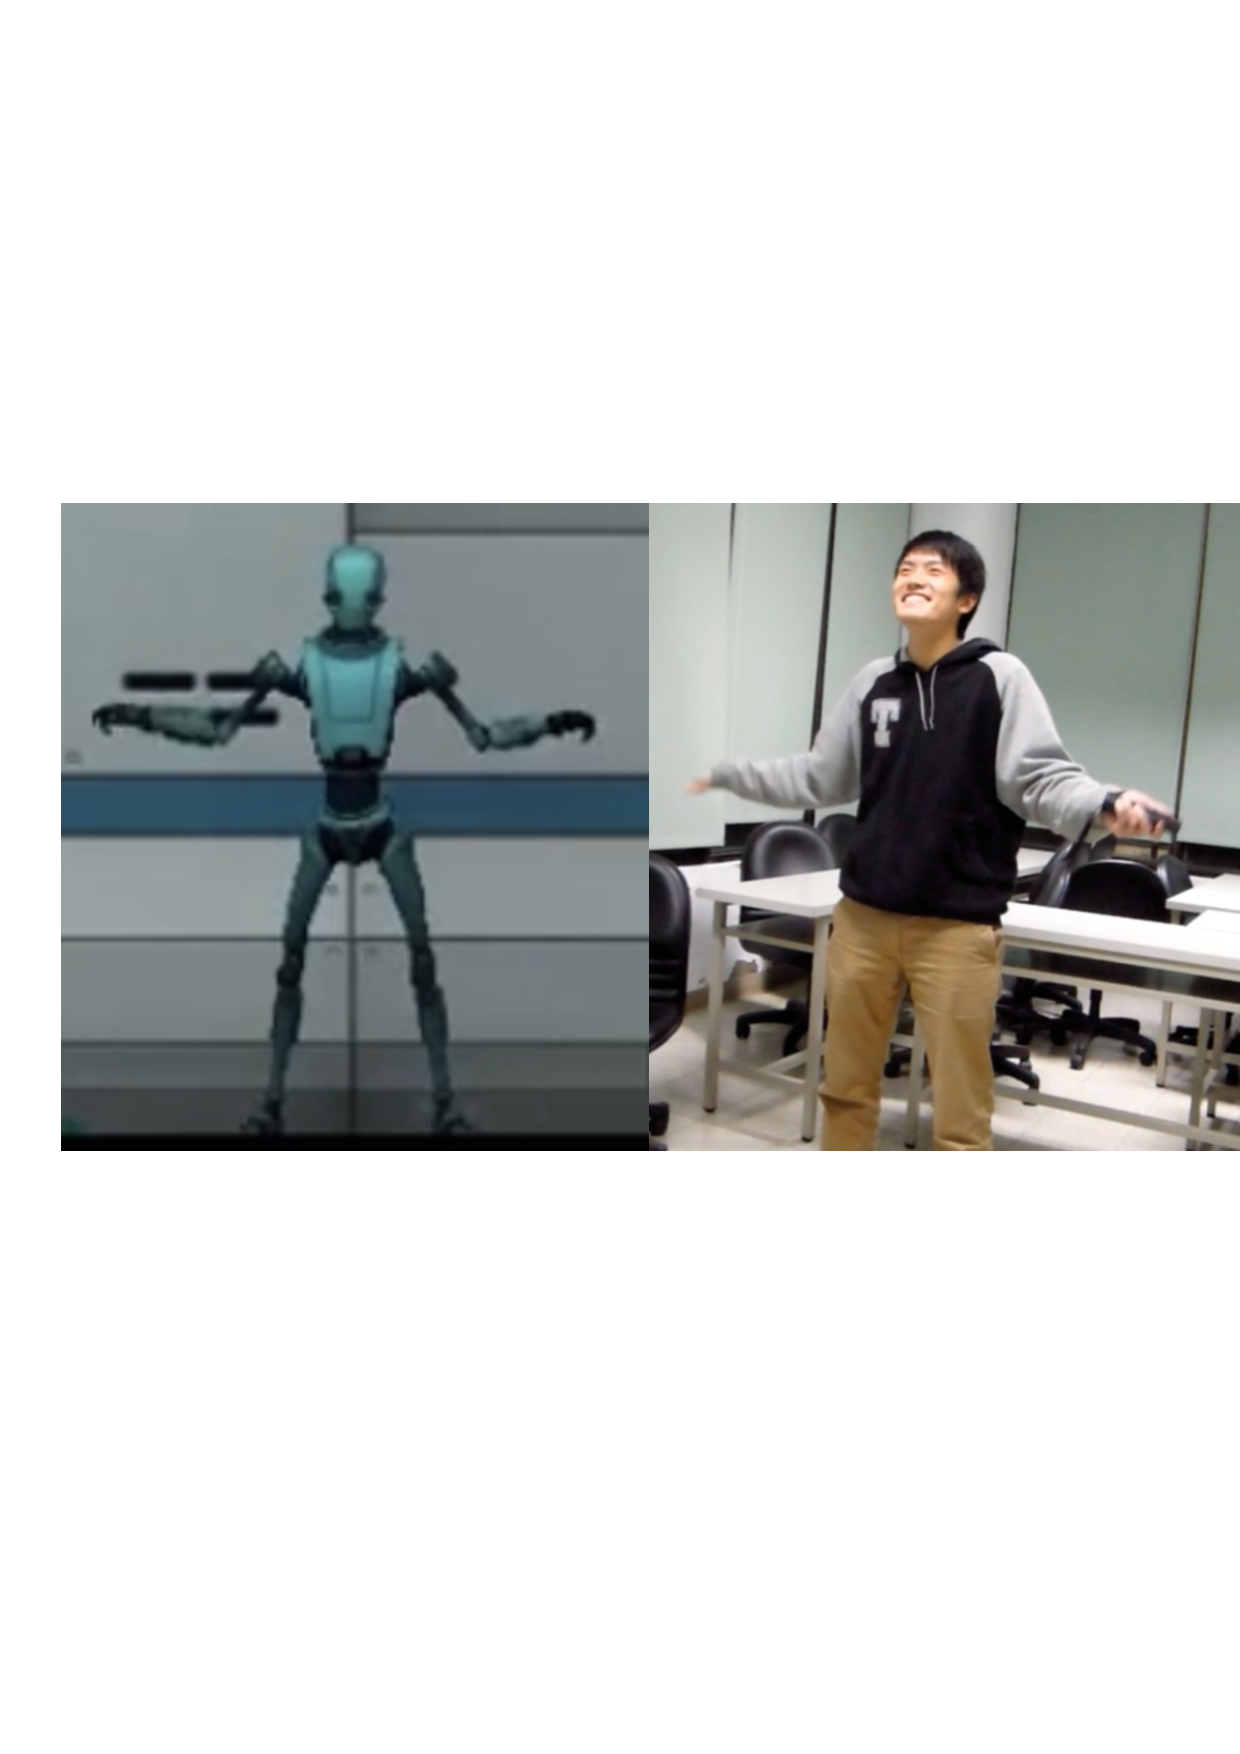
\includegraphics[width=1.0\columnwidth]{Figures/GD_F1.pdf}
\caption{Body movement mapping between player and avatar by Kinect}
\label{fig:GD_F1}
\end{figure}


\subsection{Game Design in Mute Robot}

For the goal to confirm our thoughts, our game design in Mute Robot match the game goal we proposed above.
\begin{enumerate}
\item Focus on Communication : 
in order to strengthen the necessarily of communication between players, we manufacture ``Informatin asymmetric'' environment, which means that one player will receive some messages, and he needs to transfer messages to another player through communication (see Figure \ref{fig:GD_F2}). This will enforce players to communicate with each other. In our game, we also switch the player with receiving messages, so players will take turn to take over messages and make communicate in both directions. In order to make players communicate without distraction, we let the avatar, which corresponds to players movement in our game, catch player's body language when the player is not moving. In other words, player's body motion won't map to the avatar when the avatar is moving.
% 為了加強玩家間溝通的必要性,我們使用了Information asymmetric的設計,讓玩家間獲得的資訊不一致,擁有資訊的人必須透過溝通將訊息傳遞給其他人,this will make players communicate with each other 強制性地.在遊戲中,掌握資訊的玩家會交換,使得溝通不會只有單一方向,而會是交錯式的溝通方式。為了不讓玩家在溝通時分散注意力,我們在虛擬角色靜止不動時才抓玩家肢體語言,在角色移動時並不會map 玩家的動作。

\item Test the limitation: in order to test the limitation of using body language in cooperative game, we designed three puzzles with incremental difficulty. It means that the message player received will have higher complexity than the previous one.
We also anticipate players who can express the abstract concept. All puzzle in each level will not tell players how to express, and let players imagine without any constraint.
% 在遊戲裡我們希望使用者可以表達像是情緒等抽象概念,而且每個謎題並不會告訴玩家要如何表達,讓玩家能自由發揮想像力。
\item Cooperative Fun: 
in Mute Robot, players need to interact with each other to pass the level through body language. During the game, they have to guess another player's meaning of expression until they build up an unspoken consensus with each other. Through the process of guessing, players will produce the emotional connection. And at the end of the game, we will let players have a hug with each other in a virtual game environment to express the emotional appreciation and gratefulness.
% 在Mute Robot中,玩家會透過肢體語言互動來合作過關,在遊戲過程中互相猜測對方想表達的意思,直到建立彼此的默契,透過猜測的過程了解對方,產生情感上的聯結,並在遊戲最後讓雙方以虛擬的方式擁抱,向對方表達感謝以及鼓勵。
In Mute Robot, players need to use body language to transmit messages and solve puzzles. In the beginning of the game, we observed that players attempt to guess the meaning of their partners’ postures until they build up their own understanding. 
\item Avoid Frustration: 
let players communicate through body language and descend the matter of language barrier. In Mute Robot, player just has to transmit one single object or mission at one time, with the design of incremental difficulty, to decrease the players feeling of frustration.
% 讓玩家透過肢體語言溝通,降低語言不通的問題,而且在遊戲中,我們一次只會讓玩家表達單一的東西或指令,並以漸進式的難度設計,降低玩家感到挫折的機會。
\item University: 
in our game design, we will try our best to avoid body language which is related to culture or language characteristic, and let everyone can enjoy and entertain Mute Robot.
% in our game design,我們儘量避免使用帶有文化或是語言特色的肢體語言,讓所有人都可以享受Mute Robot來的樂趣。
\end{enumerate}


\begin{figure}[!h]
\centering
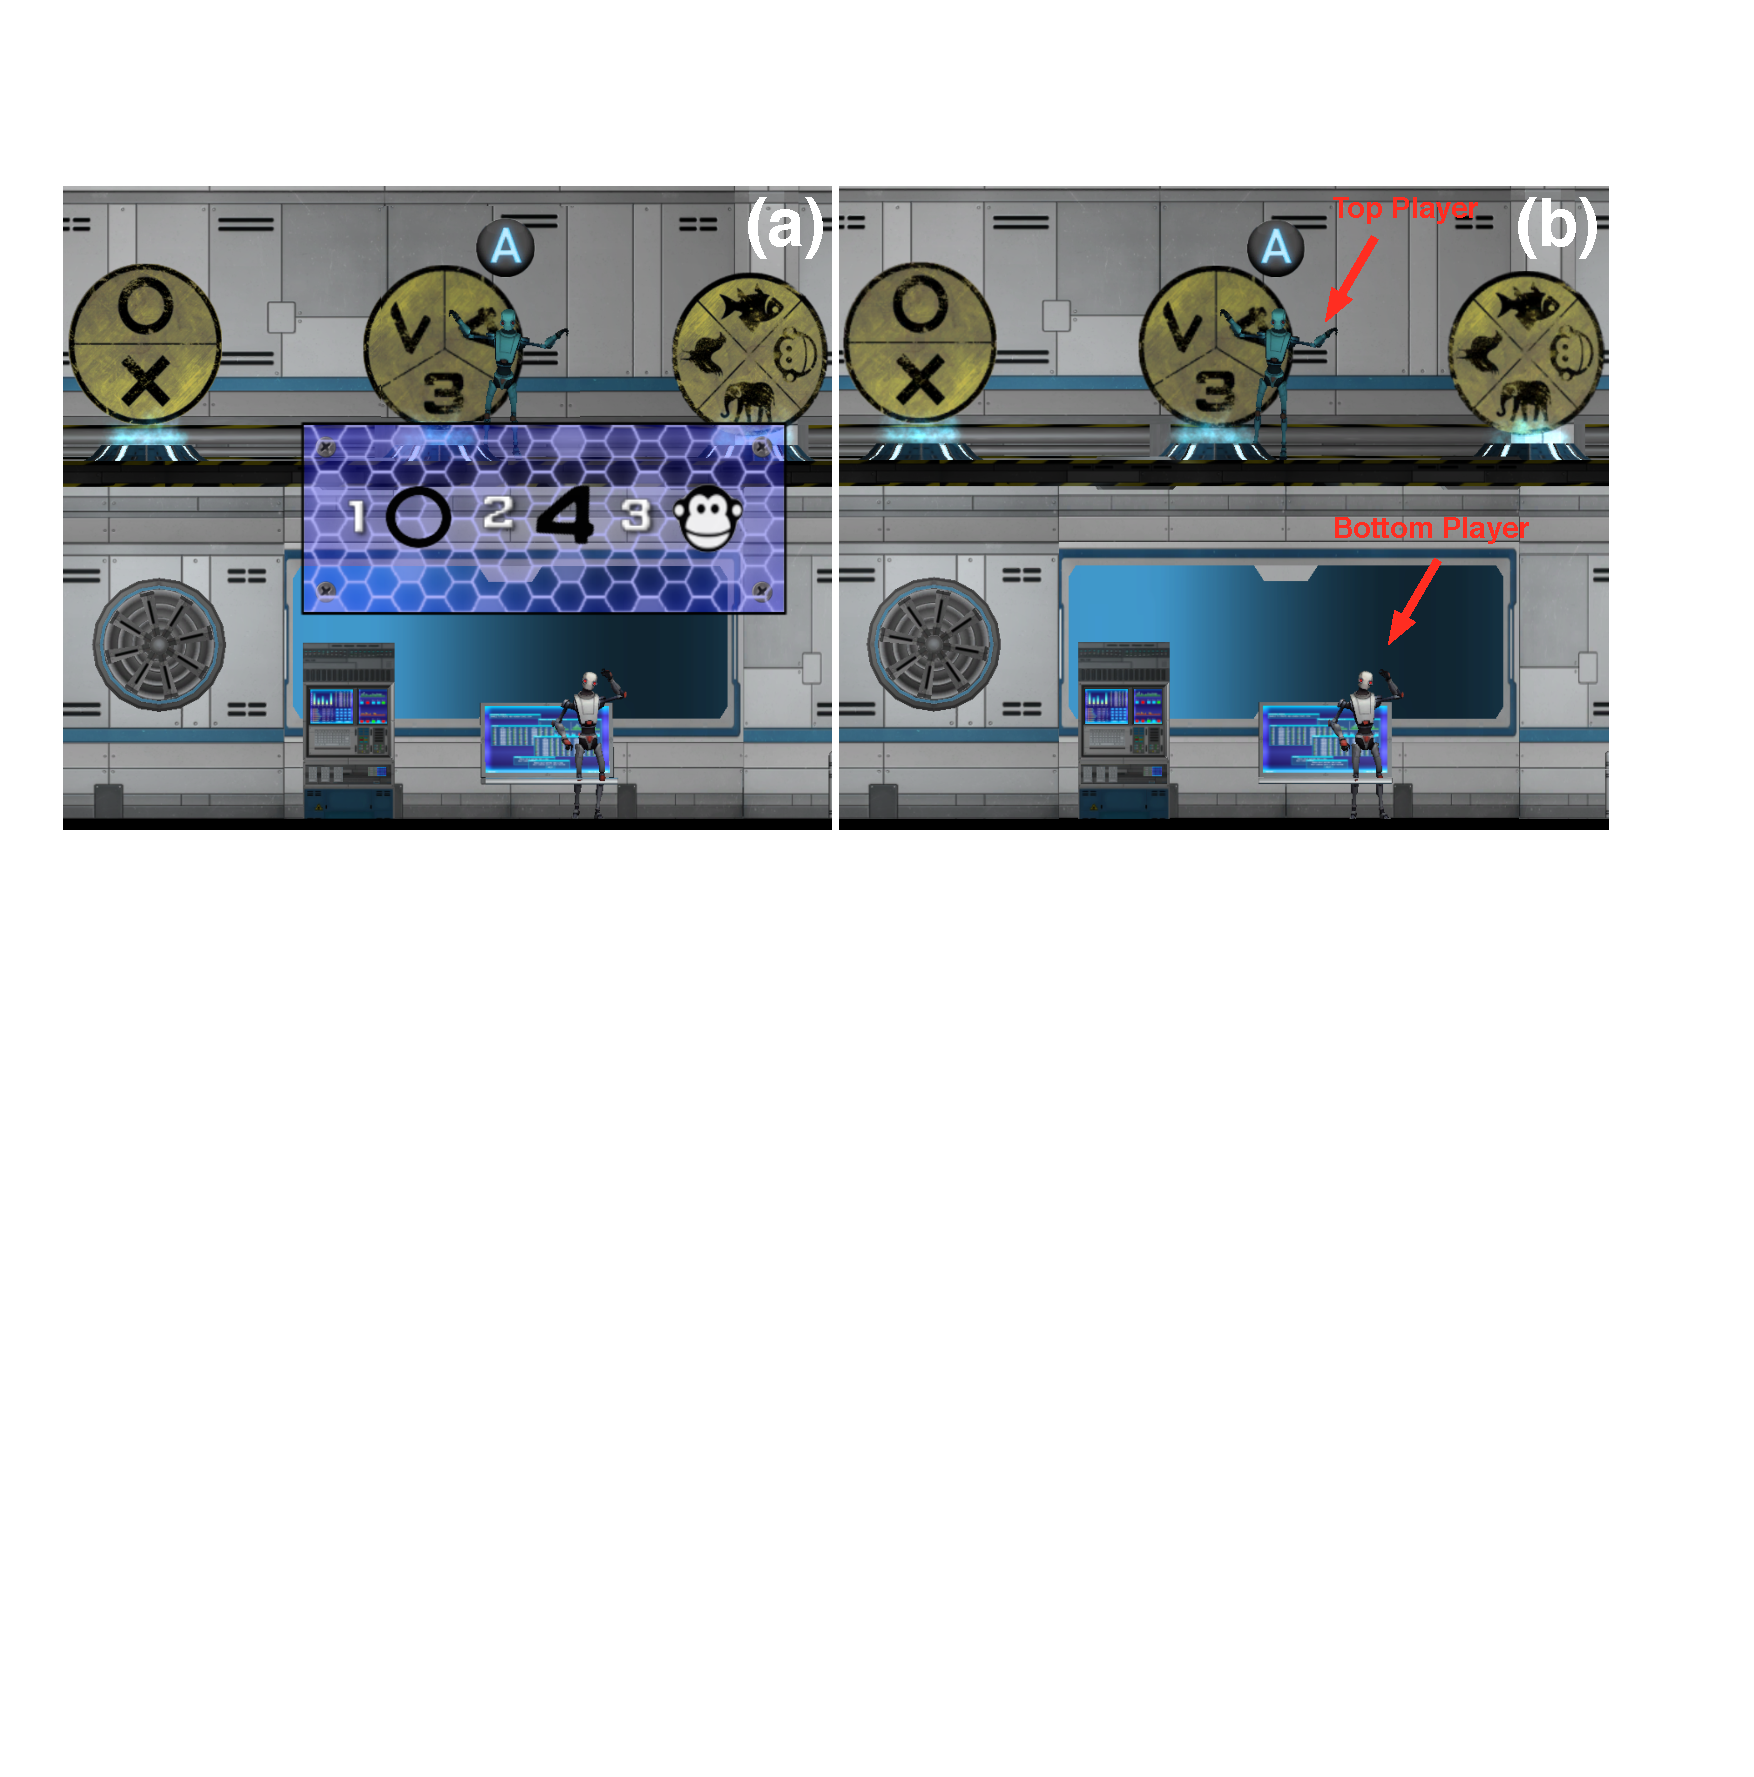
\includegraphics[width=1.0\columnwidth]{Figures/GD_F2.pdf}
\caption{The asymmetric puzzle game design in one of Mute Robot's stages. (a) Bottom player's view, (b) Top player's view}
\label{fig:GD_F2}
\end{figure}

\section{User Study}

To evaluate our game design, we totally recruited 24 groups with 48 users (33 males and 15 females, average age is 22.6) to play Mute Robot.  Every team had two players and be placed in two distinct rooms. Players played Mute Robot with each other through Internet connection. After playing Mute Robot, players filled out an extended Short Feedback Questionnaire (eSFQ) \cite{eSFQ} questionnaire to evaluate the game experience. It needs about 30 minutes to finish our user study experiment. 

\subsection{eSFQ Results}

eSFQ \cite{eSFQ} had been proved that it was a questionnaire for rapid assessment of game experience. eSFQ capture the experienced fun/enjoyment, curiosity, and co-experience. 

Fun/enjoyment included the rating of game enjoyment and the description of game experience (users selected keywords about their feeling), curiosity showed that the users were curious about the games (on a scale of 1 to 5), and co-experience were the feeling of interacting with each other (users selected keywords about their feeling).

\subsubsection{Fun and Enjoyment}
For the game fun/enjoyment, the mean level of the fun experience for Mute Robot was 4.5 (SD = 0.65) (5 meaning “Yeah, fun” - highest level of fun and 1 meaning “Yawn, boring” - lowest level of fun). Their game experiences were related to intuitive (54\% of the users), exciting (46\%), and great (33\%). 

\subsubsection{Curiosity}
Curiosity about Mute Robot was rated with a mean of 4.25 (SD = 0.85 (5 meaning very curious and 1 meaning not curious at all).

\subsubsection{Co-experience}

\begin{figure}[!h]
\centering
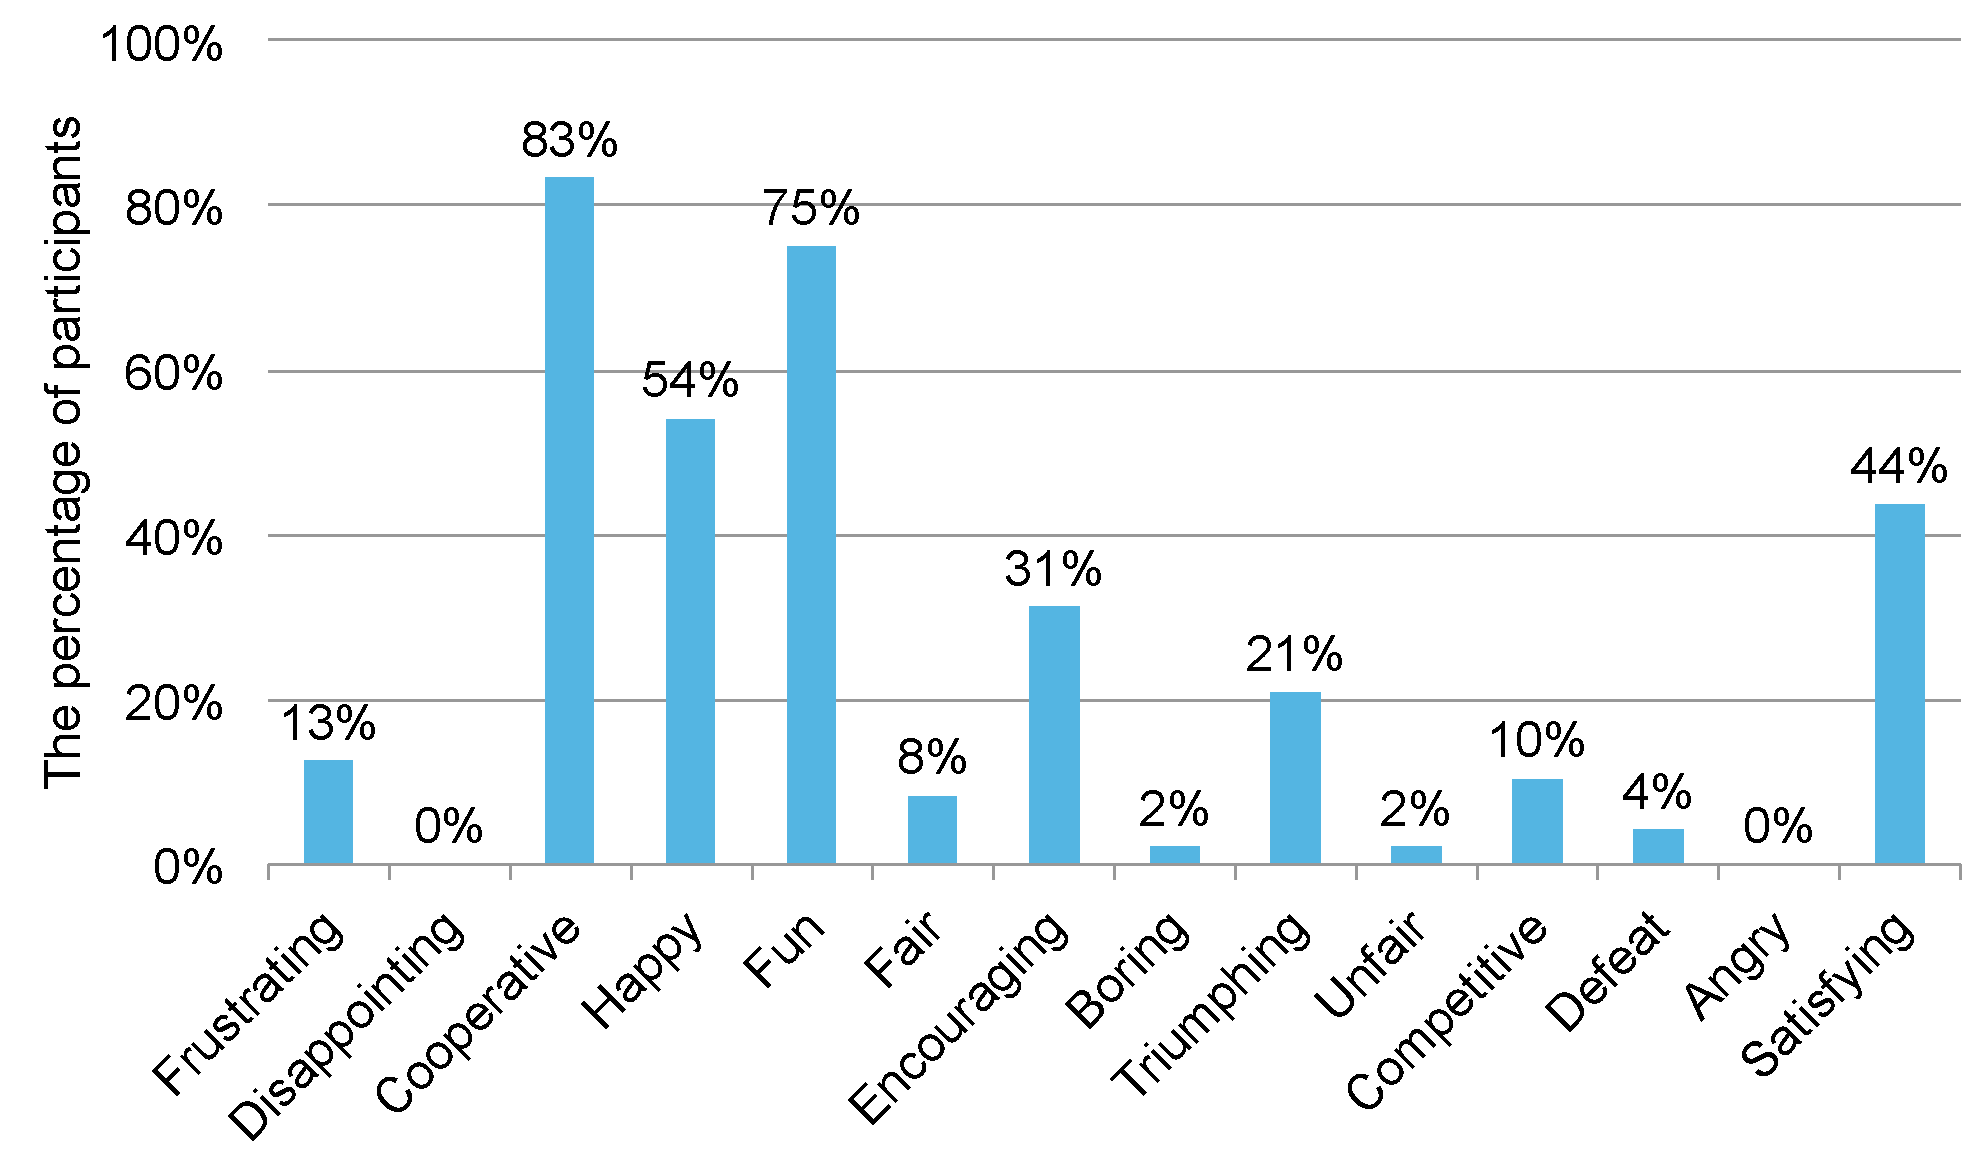
\includegraphics[width=1.0\columnwidth]{Figures/US_F1.pdf}
\caption{Co-experience indexes for players}
\label{fig:US_F1}
\end{figure}

For the game co-experience(See figure \ref{fig:US_F1}), the users experienced playing Mute Robot together as cooperative (83\% of the users), fun (75\%), happy (54\%), satisfying (44\%), and encouraging (31\%). 

%小解釋result

According to user study results, players thought Mute Robot is very interesting, and have enough curious about the game world. For co-experience, it has a good rating in cooperative, fun, happy, satisfying and encouraging. It could be said that Mute Robot has a great game experience by players evaluation. 

% 根據實驗結果,可以發現玩家認為此遊戲是十分有趣的,而且對於遊戲擁有足夠的好奇心,在co-experience方面,擁有很好的cooperative, fun, happy, satisfying, encouraging,可以說在玩家的評價下mute robot是一款十分不錯且成功的遊戲。

\section{Summary}

After user study, we extended our design goals and proposed the game design guideline for body language communication in cooperative gameplay.

\begin{enumerate}
\item Necessarily of communication: 
it's necessary for players to communicate during the game. In our game design, players need to communicate with each other in order to solve the puzzle and pass each level. In addition, the main idea of the game is communication rather than manipulation.
\item Intertwining communication environment: while players are playing the game, communication should not always be in one single direction. For example, if the upper side players always receive the message and he always needs to send the messages rather than receive the message, it becomes a terrible situation. In other words, players communication in both direction is a better game play environment and enhance the game play experience.
\item Imagination inspired:
there are many messages need to be transferred between players during the game. If sometimes we provide abstract messages for players, and without obvious telling players how to express these messages. Maybe players can imagine by their own, and they can inspire more imagination while playing the game.
\item Expression ability:
in order to consider the expression of using body language, we will not let players to transfer too many and too complex messages at one time.
\item Concentrated:
don't let players have many missions at the same time. For example, using body language to communicate and moving the avatar in a virtual game environment at the same time is not a good situation and will not produce a better game play experience.
\item Balance of physical strength:
don't let all puzzle need to be solved by body movement. It will result in too much burden for players' physical power.
\item Vocalization: 
because of the silent environment by using body language to communicate, if there is more vocal stimulation provided, it will become and construct a vigorous and entertaining environment.
\item Virtual intimacy:
under the design of interaction, we need to consider the body interaction between players, such as hand hold, embrace, hand clapping, etc. With these interaction, they will also enhance the collaboration between players.
\item Display setting: 
players have to obviously see them and another player's body movement on the display.
\item University:
with consideration of cultural distinction and different comprehension of body language, we designed to let players try their best to use universal body language.

\end{enumerate}

% (總結,正式提出design guideline,多提一些跟溝通有關的,不然跟chi movement guideline 很像)
% -  溝通必要性 : 玩家在遊戲中的溝通是必要的,必須要讓玩家透過溝通才能過關,遊戲的重點是在溝通不是在操作。
% - 交錯性:玩家間的溝通方式,應該不是單方向的溝通,而是雙方向一來一往的溝通方式。
% -  Inspire imagination : sometimes provide 抽象的訊息讓玩家傳遞,and don’t 明確告訴使用者怎麼表達,讓玩家自己去思考,激發更多想像力。
% -­ Expression Ability:考慮body language的表達能力,不要讓玩家一次表達太多以及太複雜的訊息。
% -  專一性:不要讓玩家同時做多件事,像是不該讓玩家在用body language溝通的同時移動虛擬角色。
% -
­ 體力balance : 不要所有事情都得用動作完成,會造成使用者太大的體力負荷。
% ­- Vocalization : because using body language to communicate is silent , so need to provide more 聲音刺激。
% - Virtual Intimacy : 在互動的設計上,要考慮與玩家間的肢體互動,像是牽手‘擁抱、擊掌等等,可以加強合作感。
% - 顯示設定(Display Setting):在顯示上要可以明確地看到自己和對方的肢體動作。
% - University: 考慮到文化差異對肢體語言理解的不同,儘量使用 universe body language。

\section{Conclusion and Future Work}

In this work, we proposed an innovative communication way by using body language in cooperative game design. We also completed a game prototype, Mute Robot, to evaluate and confirm our game design guideline. We conducted a user study for 24 groups within 48 users. Results indicated that body language is greatly suitable for cooperative game design, which also directly proved that our design is not only useful but also provides a better game play environment. In the future, game developers can make a better game experience with these design guidelines. 
%In addition, we hope this work can inspire more explorations of new game designs and spread game entertainment for more people.

About our future work, we will focus on improving system's sensitivity, accuracy and diversity. We are willing to use higher resolution devices or software correction. For example, using Kinect (v2) to capture player's subtle movements. Furthermore, 
%we want to capture player's facial expression that not only can we enhace the accuracy of emotional detection but we can also analyze players' emotion in more detail. Last but not least, 
we will add more different levels to increase game's diversity, and hope to spread game entertainment for more people.

\balance

%\section{References format}
%References must be the same font size as other body text.
% REFERENCES FORMAT
% References must be the same font size as other body text.

\bibliographystyle{acm-sigchi}
\bibliography{sample}
\end{document}
